
Write a function that defines $f(x) = (\sin(x) + 1)^{\sin(\cos(x))}$ and takes its symbolic derivative with respect to $x$ using SymPy.
Lambdify the resulting function so that it can accept NumPy arrays and return the resulting function handle.
% returns the derivative of $e^{\sin\left(\cos\left(x\right)\right)}$ at $x=1$ as a float using SymPy.

To check your function, plot $f$ and its derivative $f'$ over the domain $[-\pi, \pi]$.
It may be helpful to move the bottom spine to $0$ so you can see where the derivative crosses the $x$-axis.
\begin{lstlisting}
>>> from matplotlib import pyplot as plt

>>> ax = plt.gca()
>>> ax.spines["bottom"].set_position("zero")
\end{lstlisting}
% >>> for label in ["right", "top"]:      # Turn other spines off.
% ...     ax.spines[label].set_visible(False)
% ...
% \end{lstlisting}
\label{prob:sympy-symbolic-diff}
 % Implement finite difference quotients.
Write a function for each of the finite difference quotients listed in Table \ref{table:finite-difference-quotients}.
Each function should accept a function handle $f$, an array of points \li{x}, and a float $h$; each should return an array of the difference quotients evaluated at each point in \li{x}.

To test your functions, approximate the derivative of $f(x) = (\sin(x) + 1)^{\sin(\cos(x))}$ at each point of a domain over $[-\pi,\pi]$.
Plot the results and compare them to the results of Problem \ref{prob:sympy-symbolic-diff}.
\label{prob:implement-finite-difference-quotients}
 % Convergence of difference quotients.
Write a function that accepts a point $x_0$ at which to compute the derivative of $f(x) = (\sin(x)+1)^{\sin(\cos(x))}$.
Use your function from Problem \ref{prob:sympy-symbolic-diff} to compute the exact value of $f'(x_0)$.
Then use each your functions from Problem \ref{prob:implement-finite-difference-quotients} to get an approximate derivative $\tilde{f}'(x_0)$ for $h=10^{-8},10^{-7},\ldots,10^{-1},1$.
Track the absolute error $|f'(x_0) - \tilde{f}'(x_0)|$ for each trial, then plot the absolute error against $h$ on a log-log scale (use \li{plt.loglog()}).

Instead of using \li{np.linspace()} to create an array of $h$ values, use \li{np.logspace()}.
This function generates logarithmically spaced values between two powers of $10$.
\begin{lstlisting}
>>> import numpy as np
>>> np.logspace(-3, 0, 4)           # Get 4 values from 1e-3 to 1e0.
array([ 0.001,  0.01 ,  0.1  ,  1.   ])
\end{lstlisting}

For $x_0 = 1$, your plot should resemble the following figure.
\begin{figure}[H]
    \centering
    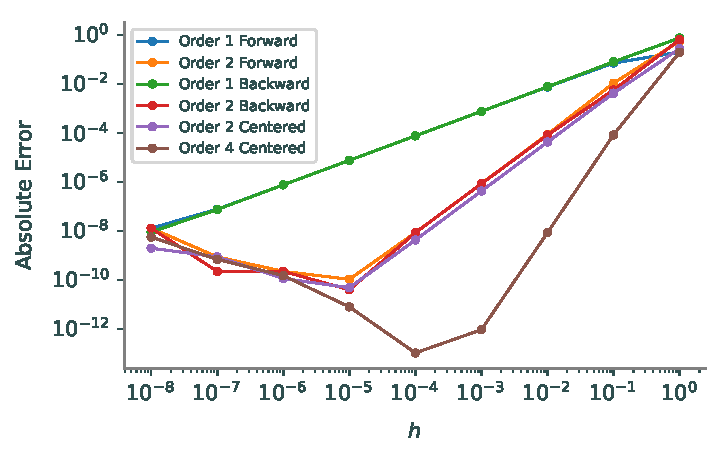
\includegraphics[width=.7\textwidth]{figures/error_plot.pdf}
\end{figure}
\label{prob:difference-quotient-convergence}

The radar stations $A$ and $B$, separated by the distance $a = 500$ m, track a plane $C$ by recording the angles $\alpha$ and $\beta$ at one-second intervals.
Your goal, back at air traffic control, is to determine the speed of the plane.
%
\begin{figure}[H]
    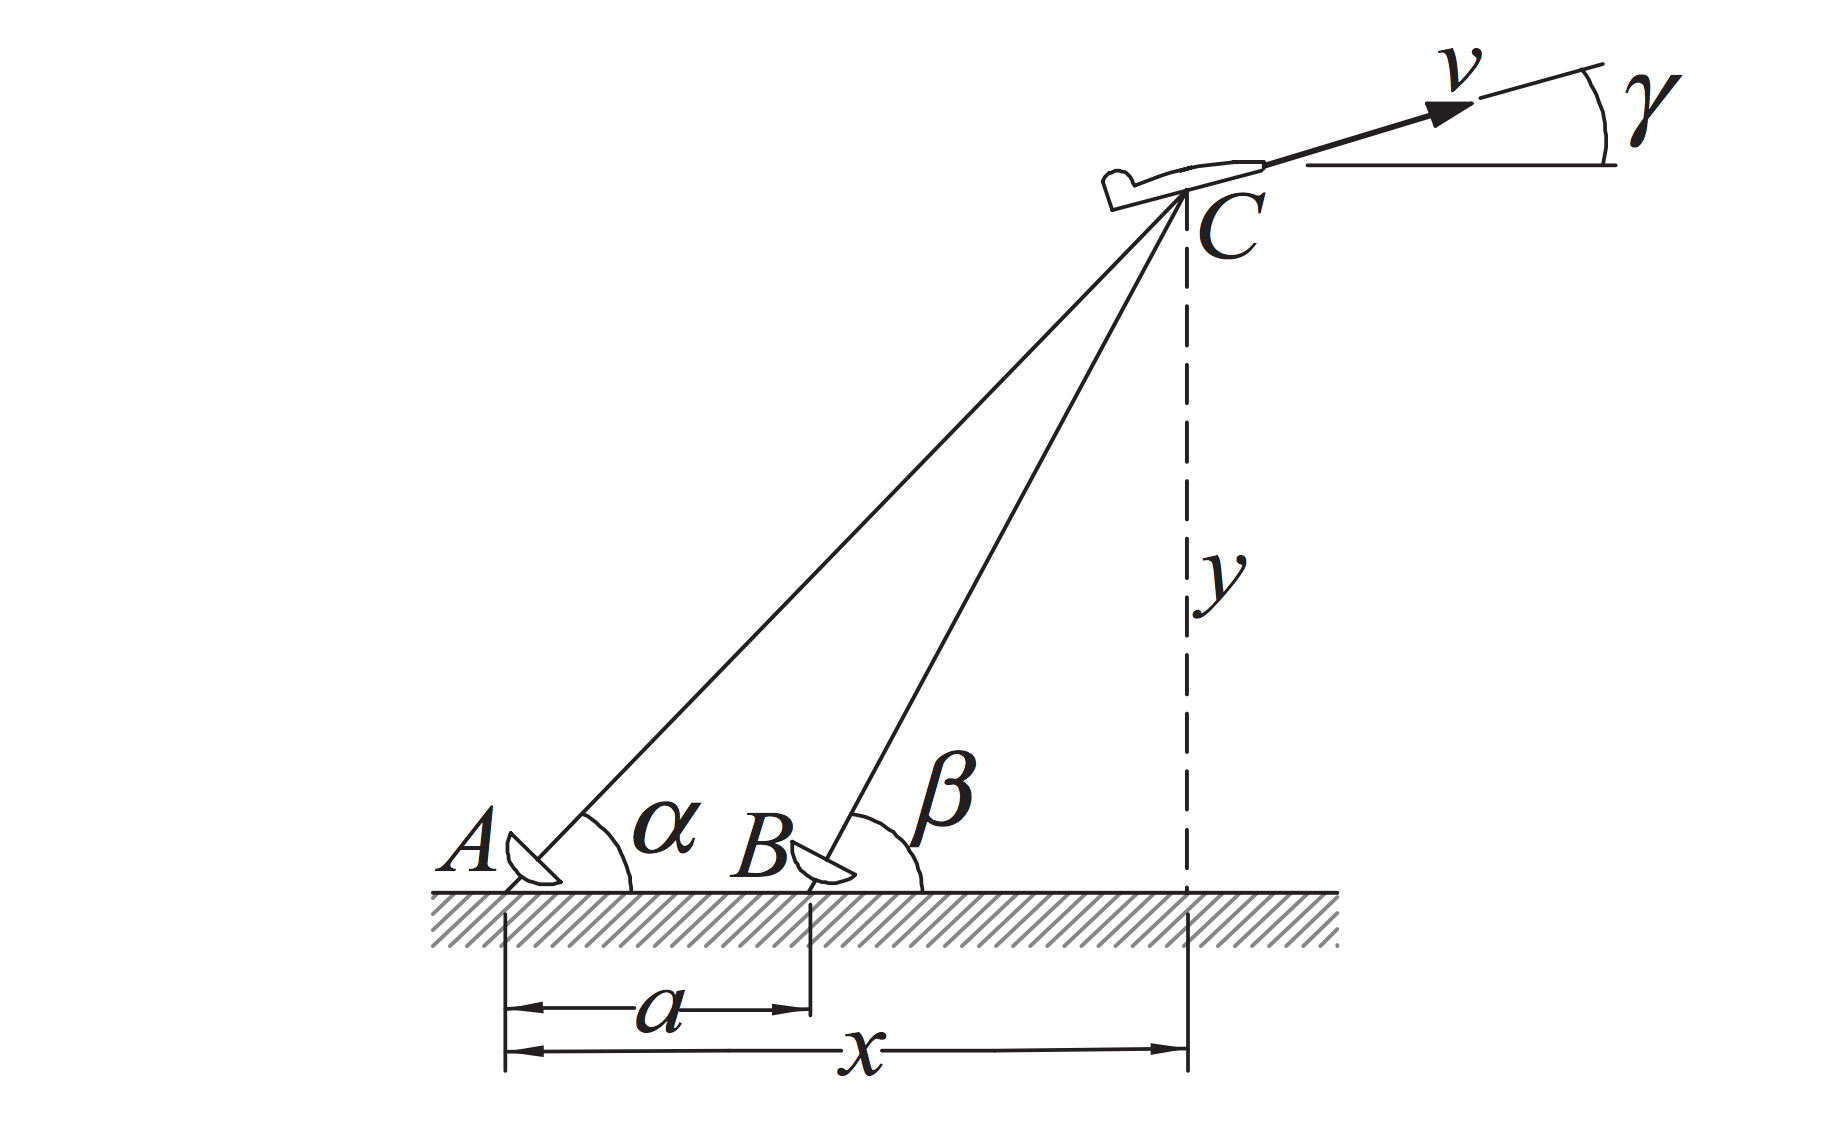
\includegraphics[width=.5\textwidth]{figures/plane_diagram.png}
\end{figure}
%
Let the position of the plane at time $t$ be given by $(x(t),y(t))$.
The speed at time $t$ is the magnitude of the velocity vector, $\|\frac{d}{dt}(x(t),y(t))\| = \sqrt{x'(t)^2 + y'(t)^2}$.
The closed forms of the functions $x(t)$ and $y(t)$ are unknown (and may not exist at all), but we can still use numerical methods to estimate $x'(t)$ and $y'(t)$.
For example, at $t=3$, the second order centered difference quotient for $x'(t)$ is
\[
x'(3) \approx \frac{x(3+h) - x(3-h)}{2h} = \frac{1}{2}(x(4) - x(2)).
\]
In this case $h=1$ since data comes in from the radar stations at $1$ second intervals.

Successive readings for $\alpha$ and $\beta$ at integer times $t=7,8,\ldots,14$ are stored in the file \texttt{plane.npy}.
Each row in the array represents a different reading; the columns are the observation time $t$, the angle $\alpha$ (in degrees), and the angle $\beta$ (also in degrees), in that order.
The Cartesian coordinates of the plane can be calculated from the angles $\alpha$ and $\beta$ as follows.
\begin{equation}
\label{eq:differentiation-plane-conversion}
x(\alpha, \beta) = a \frac{\tan(\beta)}{\tan(\beta)-\tan(\alpha)}
\qquad
y(\alpha, \beta) = a \frac{\tan(\beta)\tan(\alpha)}{\tan(\beta)-\tan(\alpha)}
\end{equation}
Load the data, convert $\alpha$ and $\beta$ to radians, then compute the coordinates $x(t)$ and $y(t)$ at each given $t$ using \ref{eq:differentiation-plane-conversion}.
Approximate $x'(t)$ and $y'(t)$ using a forward difference quotient for $t=7$, a backward difference quotient for $t=14$, and a centered difference quotient for $t=8,9,\ldots,13$ (see Figure \ref{fig:difference-quotient-grid}).
Return the values of the speed $\sqrt{x'(t)^2+y'(t)^2}$ at each $t$.\footnote{This problem originates from \emph{Numerical Methods in Engineering with Python 3} by Jaan Kiusalaas.}
\\(Hint: \li{np.deg2rad()} will be helpful.)

Write a function that accepts a function $f:\mathbb{R}^n\rightarrow\mathbb{R}^m$, a point $\x_0 \in \mathbb{R}^n$, and a float $h$.
Approximate the Jacobian matrix of $f$ at $\x$ using the second order centered difference quotient in (\ref{eq:centered-quotient-high-dimension}).
\\(Hint: the standard basis vector $\e_j$ is the $j$th column of the $n\times n$ identity matrix $I$.)

To test your function, define a simple function like $f(x,y) = [x^2, x^3 - y]\trp$ where the Jacobian is easy to find analytically, then check the results of your function against SymPy or your own scratch work.
\label{prob:jac_center}

Find the error between your Jacobian function and the analytically computed derivative on the square $[-1,1] \times [-1,1]$ using ten thousand grid points (100 per side).
You may apply your Jacobian function to the points one at a time using a double \li{for} loop.  Once you get the error matrix for a given point, calculate the Frobenius norm of this matrix (\li{la.norm()} defaults to the Frobenius norm).  This norm will be your total error for that point.
Return the maximum error of your Jacobian function over all points in the square.

Hint: The following code defines the function
$f(x,y) = \left[\begin{array}{c} x^2 \\ x+y \end{array}\right]$.

\begin{lstlisting}
# f accepts a length-2 NumPy array
>>> f = lambda x: np.array([x[0]**2, x[0]+x[1]])
\end{lstlisting}
 % Take the derivative of a recursive function.
The \emph{Chebyshev Polynomials} are recursively defined as follows.
\[
T_0(x) = 1\qquad T_1(x) = x\qquad T_n(x) = 2xT_{n-1}(x) - T_{n-2}(x)
\]
Write a function that accepts an array $x$ and an integer $n$ and recursively computes $T_n(x)$.
Use Autograd and your first function to create a function for $T_n'(x)$.
Use this last function to plot each $T_n'(x)$ over the domain $[-1, 1]$ for $n=0,1,2,3,4$.
\\(Hint: Use \li{anp.ones_like(x)} to handle the case when $n = 0$.)
 % Compare differentiation methods.
Let $f(x) = (\sin(x) + 1)^{\sin(\cos(x))}$ as in Problems \ref{prob:sympy-symbolic-diff} and \ref{prob:difference-quotient-convergence}.
Write a function that accepts an integer $N$ and performs the following experiment $N$ times.
\begin{enumerate}
\item Choose a random value $x_0$.
\item Use your function from Problem \ref{prob:sympy-symbolic-diff} to calculate the ``exact'' value of $f'(x_0)$.
Time how long the entire process takes, including calling your function (each iteration).
\item Time how long it takes to get an approximation $\tilde{f}'(x_0)$ of $f'(x_0)$ using the fourth-order centered difference quotient from Problem \ref{prob:difference-quotient-convergence}.
Record the absolute error $|f'(x_0) - \tilde{f}'(x_0)|$ of the approximation.
\item Time how long it takes to get an approximation $\bar{f}'(x_0)$ of $f'(x_0)$ using Autograd (calling \li{grad()} every time).
Record the absolute error $|f'(x_0) - \bar{f}'(x_0)|$ of the approximation.
\end{enumerate}

Plot the computation times versus the absolute errors on a log-log plot with different colors for SymPy, the difference quotient, and Autograd.
For SymPy, assume an absolute error of \li{1e-18} (since only positive values can be shown on a log plot).

For $N=200$, your plot should resemble the following figure.
Note that SymPy has the least error but the most computation time, and that the difference quotient takes the least amount of time but has the most error.
% Autograd also has less computation time than SymPy and smaller errors than the difference quotient.

\begin{figure}[H]
    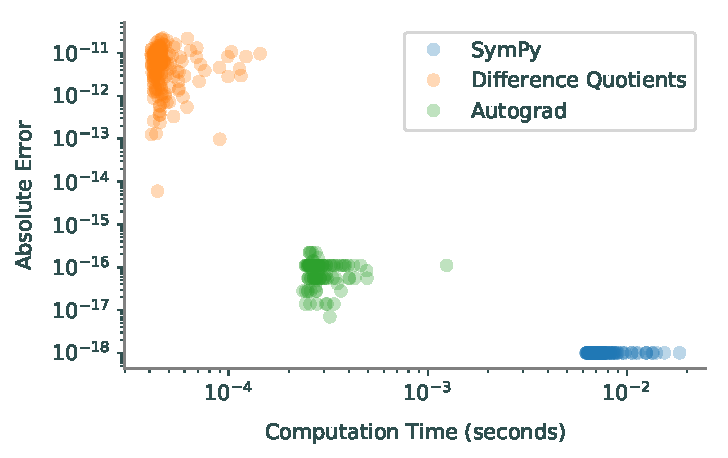
\includegraphics[width=.7\textwidth]{figures/efficiency.pdf}
\end{figure}
\label{prob:filter}
\leavevmode
Finish writing the function \li{Filter} by filling in lines 5, 6, and 10.  Hint: Note in \ref{equ:convolve}, $C_{ij}$ was calculated by summing from -1 to 1.  This is only the case if the filter \li{F} is $3 \times 3$. A slight modification is needed in the general case.  Test your function on the image \li{cameraman.jpg} using the Gaussian Blur. The result is in Figure \ref{fig:cameraman_blur}.

Write a function that accepts an image as input and applies the Sobel filter to the image.  Test your function on \li{cameraman.jpg}.  Hint: If you want to find the average of a matrix \li{A}, use the function \li{A.mean()}.
